\section{Graph Neural Networks 1}
Graphs and machine learning:
\begin{itemize}
    \item How to take advantage of the relational structure for better prediction?
    \item Many Deep Learning Approaches are designed for sequential data or grid data.
    \item Networks are more complex: Graph Deep Learning is harder
\end{itemize}
\subsection{Definition of a(heterogenous) Graph}
\(G = (V,E,R,T)\)
\begin{table}[!h]
    \begin{tabular}{lr}
    Nodes with node types    &  \(v_i \in V\)\\
    Edges with relation types     &  \((v_i,r,v_j) \in E\)\\
    Node type     &  \(T(v_i)\)\\
    Relation type     & \(r \in R\)
    \end{tabular}
\end{table}
Directed or undirected Edges
\subsection{Heterogenous Graphs}
\begin{figure}[!h]
    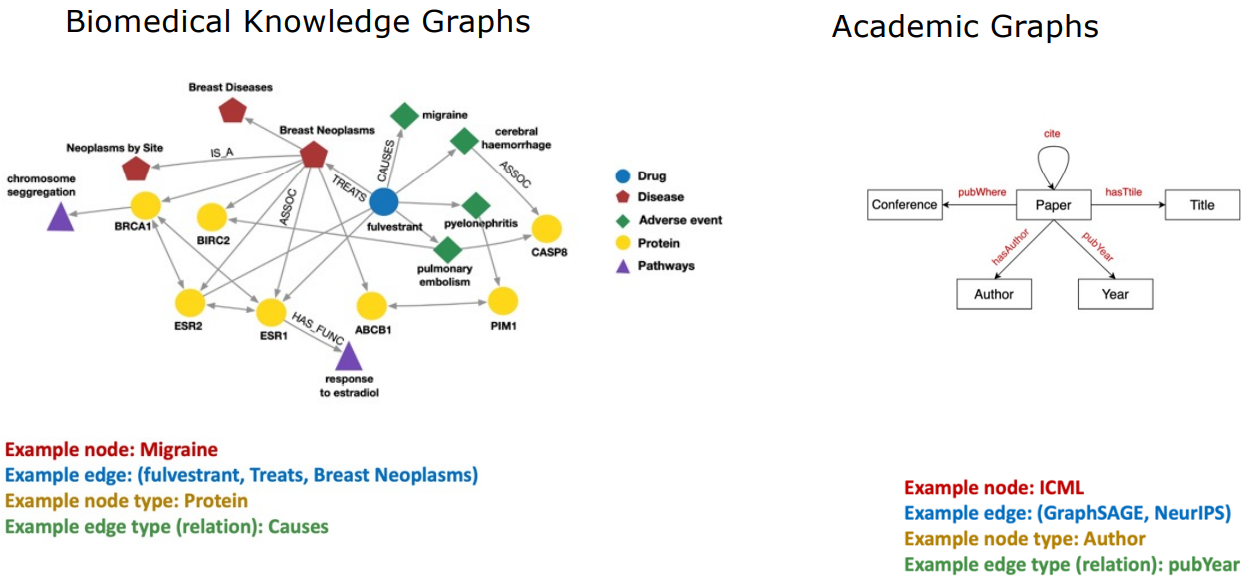
\includegraphics[width = \columnwidth]{figures/GraphNeuralNetworks1/HeterogenousGraphExample.png}
\end{figure}

\subsection{Tasks on Graphs}
Many of the problems that we would like to solve, can be described as one of several taks on graphs:
\begin{itemize}
    \item Node Level Tasks
    \item Edge Level Tasks
    \item Graph Level Tasks, Prediction / Generation
    \item Community (Subgraph) Level Taks
\end{itemize}

\subsubsection{Node Level Tasks}
Predict the identity of node in the graph.
Karate club: Predict if the student becomes loyal to Mr.Hi or Mr.John A.
\subsubsection*{Examples:}

Predict a proteins 3D structure based on its amino acid sequence:
For each node: Predict its 3D coordinates

AlphaFold:
\begin{itemize}
    \item Key idea: Spatial Graph 
    \item \textbf{Nodes:} Amino acids in a protein sequence 
    \item \textbf{Edges:} Proximity between amino acids (residues) 
\end{itemize}

\subsubsection{Edge Level Tasks}
Predict or label edges 
\subsubsection*{Examples}
Recommender System:
\begin{itemize}
    \item User interacts with items:
    \subitem Watch movies, buy merchandise, listen to music
    \item Nodes:
    \subitem Users and items
    \item Edges
    \subitem User-item interactions 
\end{itemize}
\begin{figure}[!h]
    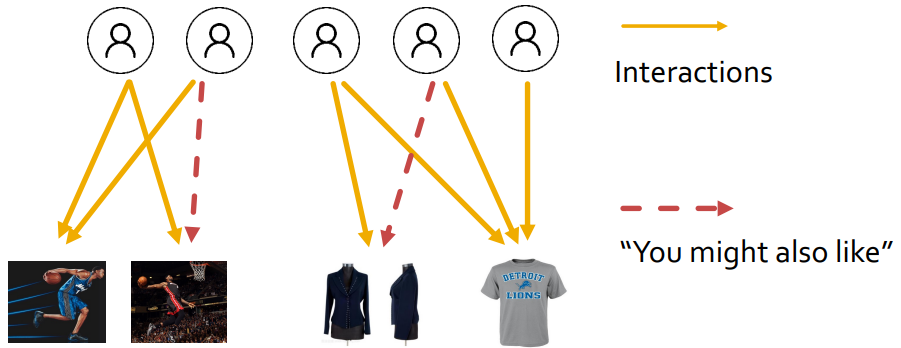
\includegraphics[width = \columnwidth]{figures/GraphNeuralNetworks1/ExampleRecommenderSystems.png}
\end{figure}
Drug Side Effects:
\begin{itemize}
    \item Nodes: Drug and proteins
    \item Edges: Interactions 
    \item Query: How likely will Simvastatin and Ciprofloxacin, when taken together, break down muscle tissue?
\end{itemize}
\begin{figure}[!h]
    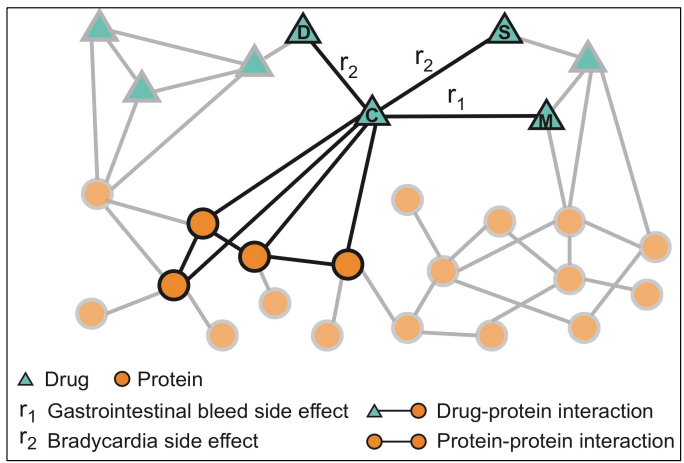
\includegraphics[width = \columnwidth]{figures/GraphNeuralNetworks1/ExampleDrugSideEffects.png}
\end{figure}

\subsubsection{Graph Level Tasks}
\subsubsection*{Examples:}
Road Network as Graph:
\begin{itemize}
    \item \textbf{Nodes:} Road segments
    \item \textbf{Edges:} Connectivity between road segments
    \item \textbf{Prediction:} Time of Arrival (ETA)
\end{itemize}
Embeddings:

Given a graph, find node, edge or graph embeddings.
Node to vector embeddings: Graph Representation Learning

Task: Map Nodes into an embedding space.
Similarity of embeddings between nodes indicate their similarity in the network. For example:
\begin{itemize}
    \item Both nodes are close to each other (connected by an edge)
    \item Encode network information
    \item Potentially used for downstream predictions
\end{itemize}
\begin{figure}[!h]
    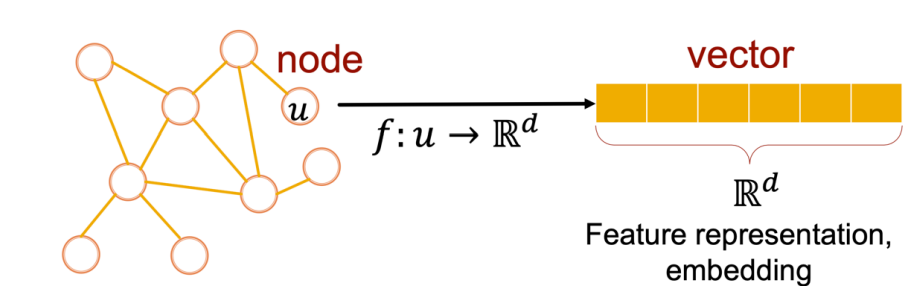
\includegraphics[width = 0.45\columnwidth]{figures/GraphNeuralNetworks1/GraphEmbedding1.png}
    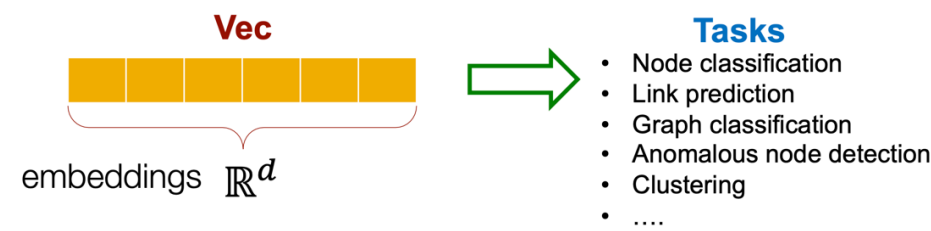
\includegraphics[width = 0.5\columnwidth]{figures/GraphNeuralNetworks1/GraphEmbedding2.png}
\end{figure}

\subsection{Challenges}
How to apply deep learning for these tasks?
Problem with how to use model connectivity!

Adjecency matrices are straight forward but:
\begin{itemize}
    \item Graphs can have millions of nodes
    \item While graphs can also have millions of edges, the matrices would be sparse
    \item Many different adjacency matrices describe the same connectivity
\end{itemize}
\subsubsection{Intuitive method}
Join adjacency matrix and features.
Feed them into deep neural network.
Problems:
\begin{itemize}
    \item Node ordering
    \item Not applicable to graphs of different sizes
    \item Oder of O(|V|) parameters 
\end{itemize}
\subsubsection{Intuitive method:CNNs?}
Generalize convolutions beyond simple lattices (image,text) ?

Graphs can look very different:
\begin{itemize}
    \item No notation of sliding window over graph \dots
    \item Graph is permutation invarant.
\end{itemize}
\subsection{Permutation Invariance and Permutation Equivariance}
Embedding of graph (or nodes) must calculate in the same result regardless of the node ordering.
Consider learning \(f\) that maps a graph \(G = (A,X)\) to a vector.
\subsubsection*{Permutation Invariance}
A graph function is \textbf{permutation invariant} if
\[
f(A,X) = f(PAP^T,PX)
\]
for and permutation \(P\).
\(A\) is the adjacency matrix.
\(X\) is the feature matrix.
\begin{figure}[!h]
    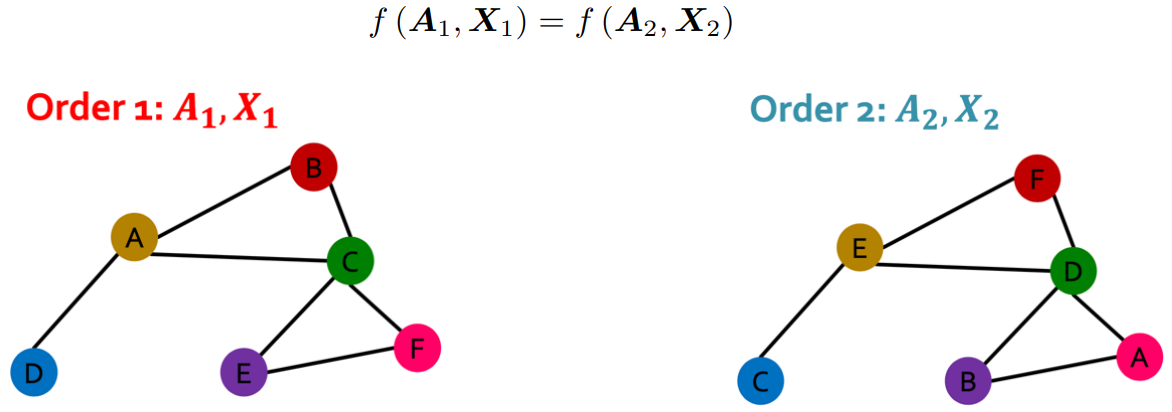
\includegraphics[width = \columnwidth]{figures/GraphNeuralNetworks1/PermutationInvariance.png}
\end{figure}
\subsubsection*{Permutation Equivariance}
A graph function is \textbf{permutation equivariant} if
\[
Pf(A,X) = f(PAP^T,PX)
\]
for and permutation \(P\).
\(A\) is the adjacency matrix.
\(X\) is the feature matrix.
\begin{figure}[!h]
    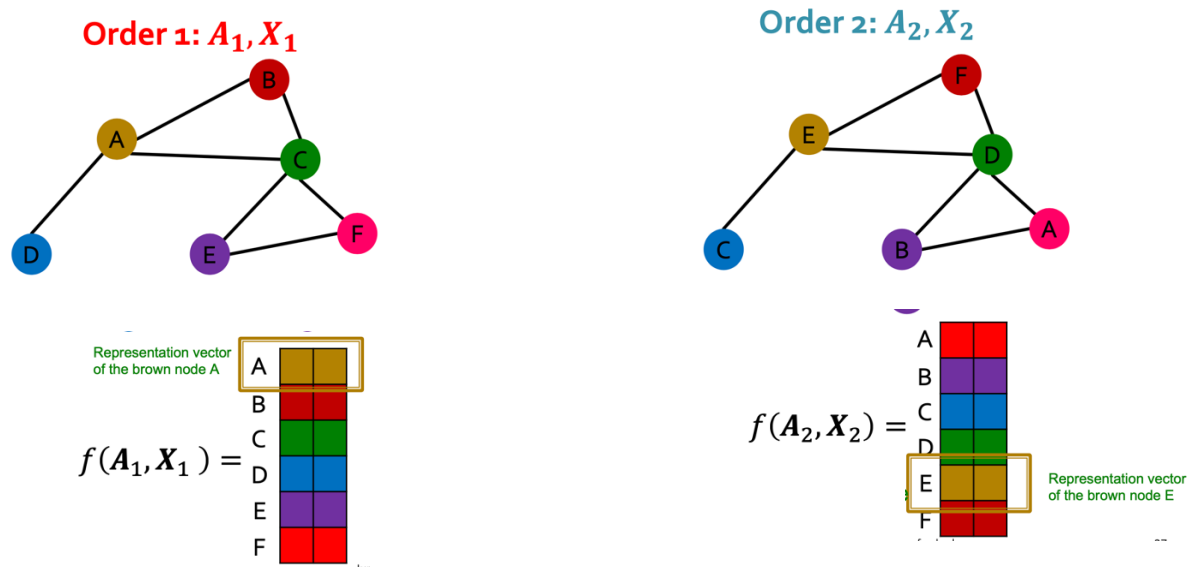
\includegraphics[width = \columnwidth]{figures/GraphNeuralNetworks1/PermutationEquivariance.png}
\end{figure}

\subsection{Representation of sparse matrices}
An \textbf{adjacency list} contains entry of each edge between nodes.
The full graph representation (with features on nodes and edges) can then be described through tensors.
\begin{figure}[!h]
    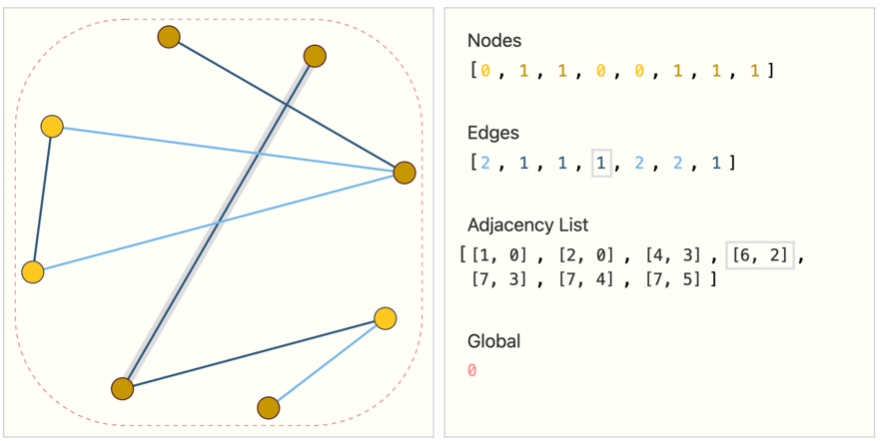
\includegraphics[width = \columnwidth]{figures/GraphNeuralNetworks1/SparseMatrices.png}
\end{figure}

\subsection{Graph Neural Networks (GNN)}
A GNN is an optimizible transformation on all attributes of the graph (nodes, edges, global-context) that preserves graph symmetries (permutation invariance)

Approach to GNNs:
\begin{itemize}
    \item Message passing neural network
    \item Graph net architecture (Graph-In, Graph-Out Model)
\end{itemize}

\subsubsection{GNNs Architecture}
Graph-In, Graph-Out Model:
\begin{itemize}
    \item Input is a graph with information in nodes, edges and global context
    \item These embeddings are continuously transformed without changing the connectivity of the input graph
\end{itemize}

\subsubsection*{A simple GNN}
Use a seperate MLP for each component (node,edge, global context) of the graph.
\begin{figure}[!h]
    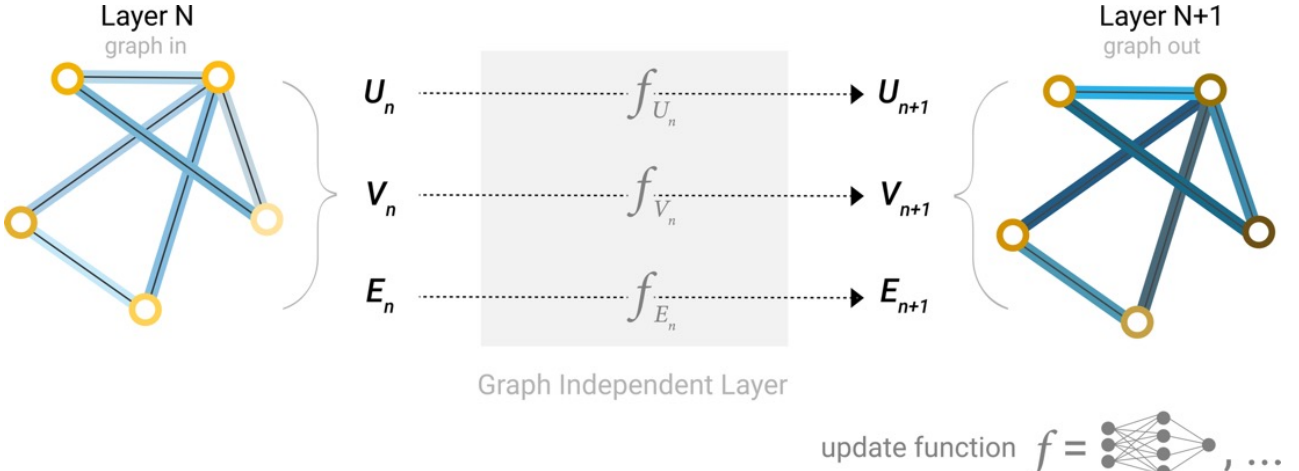
\includegraphics[width = \columnwidth]{figures/GraphNeuralNetworks1/SimpleGNN.png}
\end{figure}

\subsubsection*{Node Predictions}
Add a linear classifier after the last layer for (simple) node prediction.

\begin{figure}[!h]
    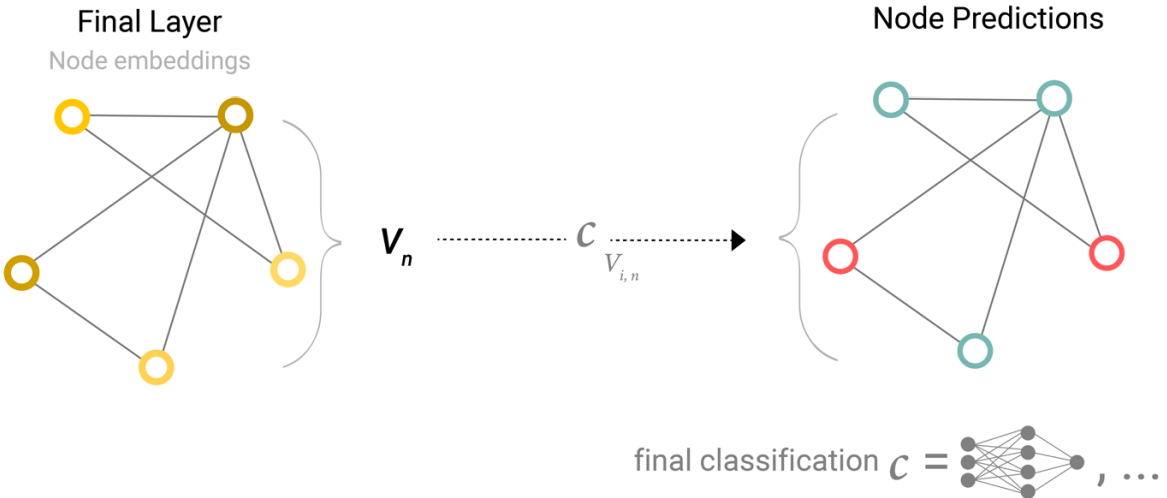
\includegraphics[width = \columnwidth]{figures/GraphNeuralNetworks1/NodePredictions.png}
\end{figure}

\subsubsection*{Node Prediction from edges}
However, we might want to use the information on the edges to make predictions on the nodes.
We can use \textbf{pooling} and \textbf{aggregation}:
\begin{figure}[!h]
    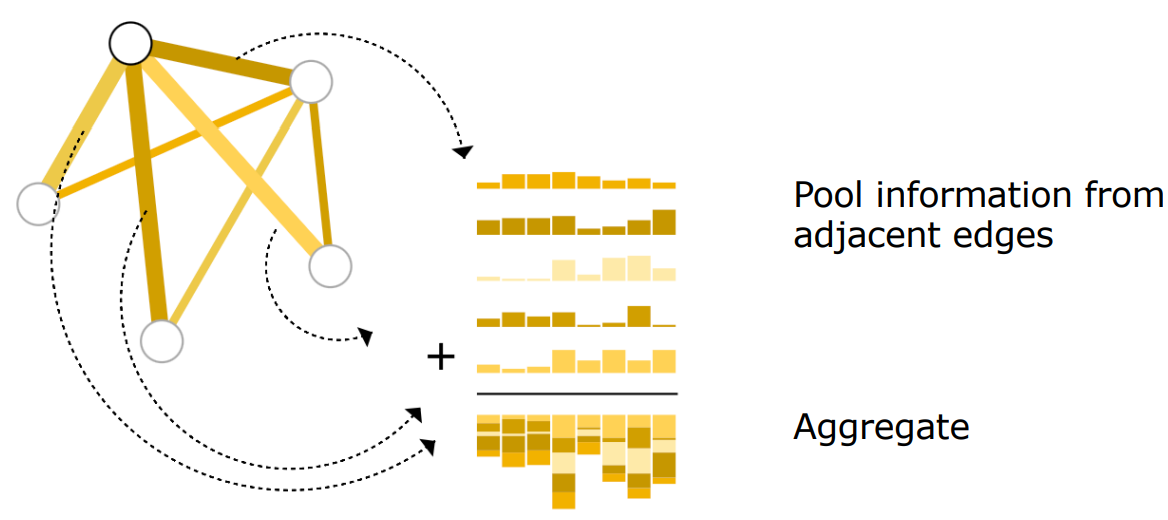
\includegraphics[width = 0.7\columnwidth]{figures/GraphNeuralNetworks1/PredictionFromEdges.png}
\end{figure}

\subsubsection*{Node Prediction from Edges only}
\begin{figure}[!h]
    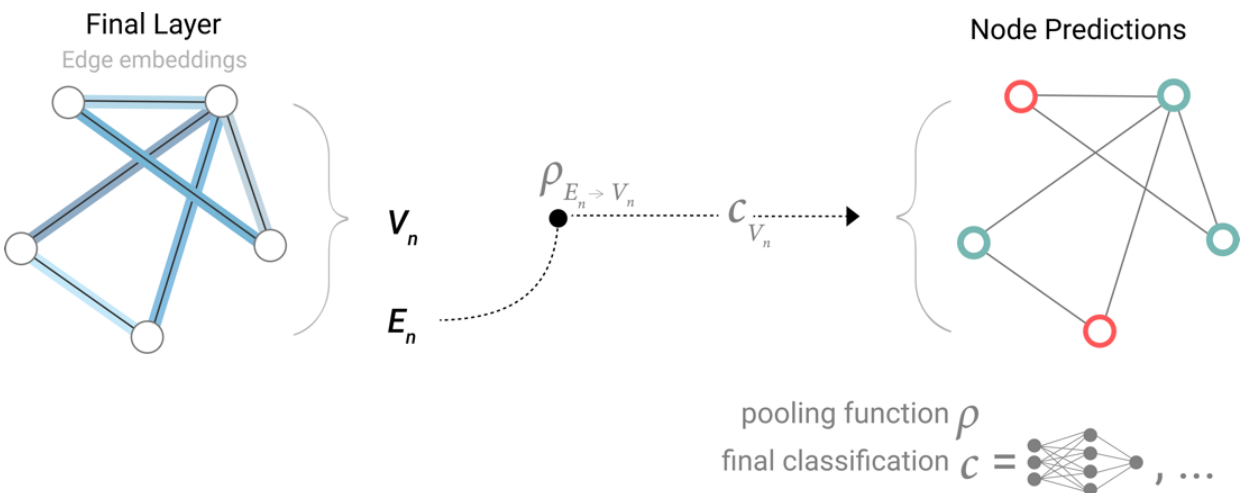
\includegraphics[width = \columnwidth]{figures/GraphNeuralNetworks1/NodePredictionFromEdgesOnly.png}
\end{figure}

\subsubsection*{Edge Prediction from Nodes (only)}
\begin{figure}[!h]
    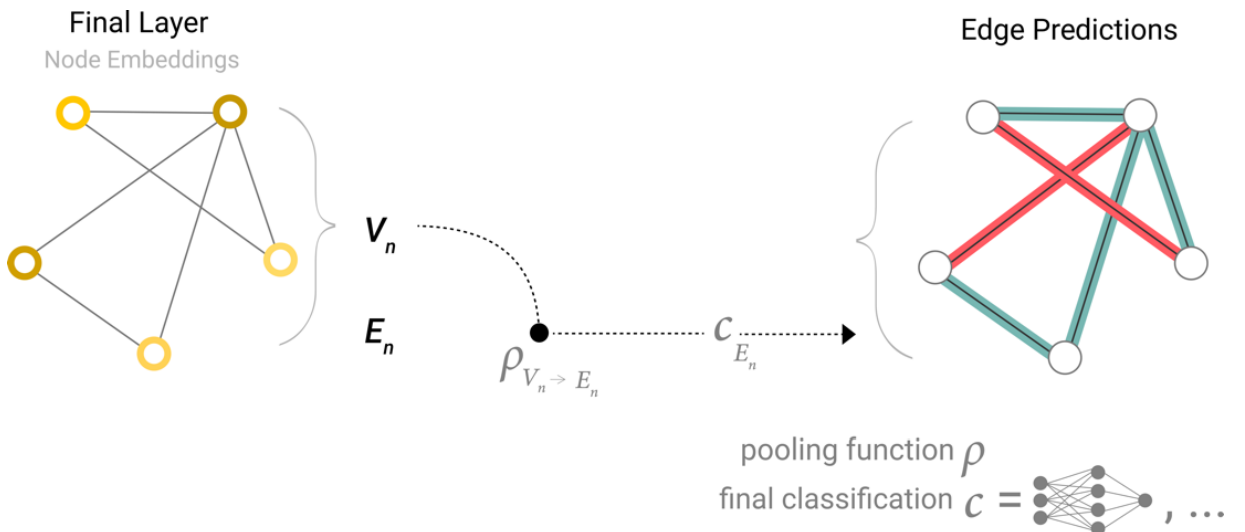
\includegraphics[width = \columnwidth]{figures/GraphNeuralNetworks1/EdgePredictionsFromNodes.png}
\end{figure}

\subsubsection*{Global Prediction}

If we want to make a global prediction, we can pool all node (or edge) information.
This is similar to pooling layers in CNNs.
\begin{figure}[!h]
    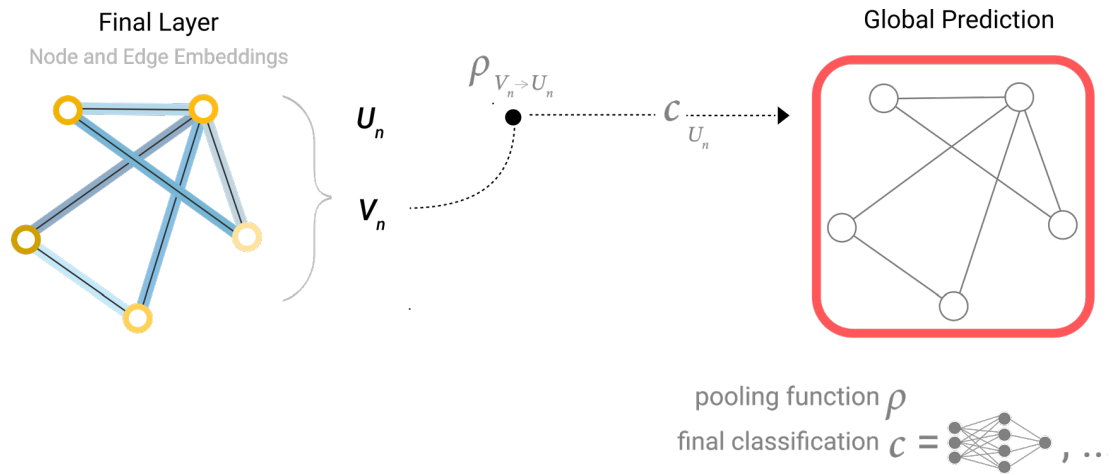
\includegraphics[width = \columnwidth]{figures/GraphNeuralNetworks1/GlobalPrediction.png}
\end{figure}

\subsubsection{Overall simple GNN}
In this simple GNN, connectivity information is only used for pooling, the nodes and edges are processed individually.
\begin{figure}[!h]
    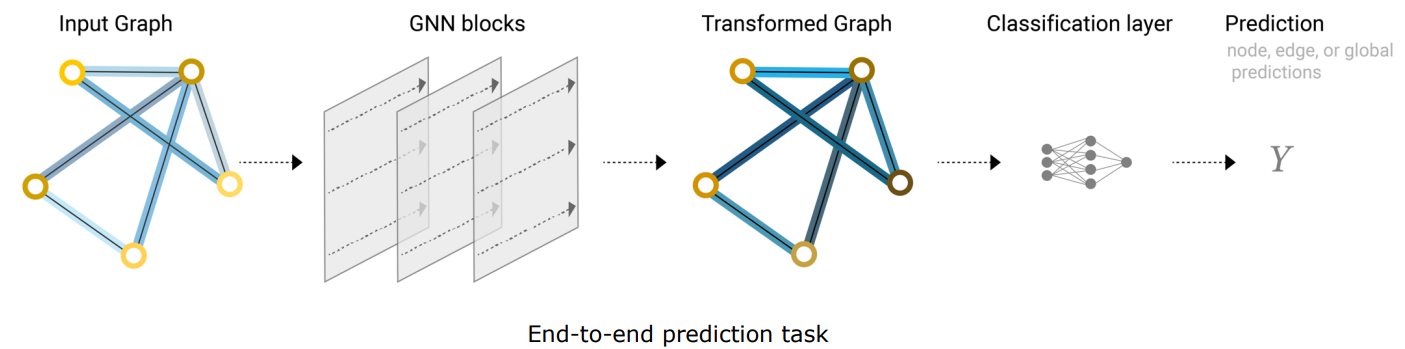
\includegraphics[width = \columnwidth]{figures/GraphNeuralNetworks1/OverallSimpleGNN.png}
\end{figure}

\subsection{Message Passing}
Neighboring nodes (or edges) are now allowed to pass messages, so that our learned embeddings are aware of the graph connectivity.

Message passing:
\begin{itemize}
    \item Gather neighboring node information (embeddings) for each node
    \item Aggregate all messages using aggregate function
    \item Pass the pooled messages through an update function 
\end{itemize}
\begin{figure}[!h]
    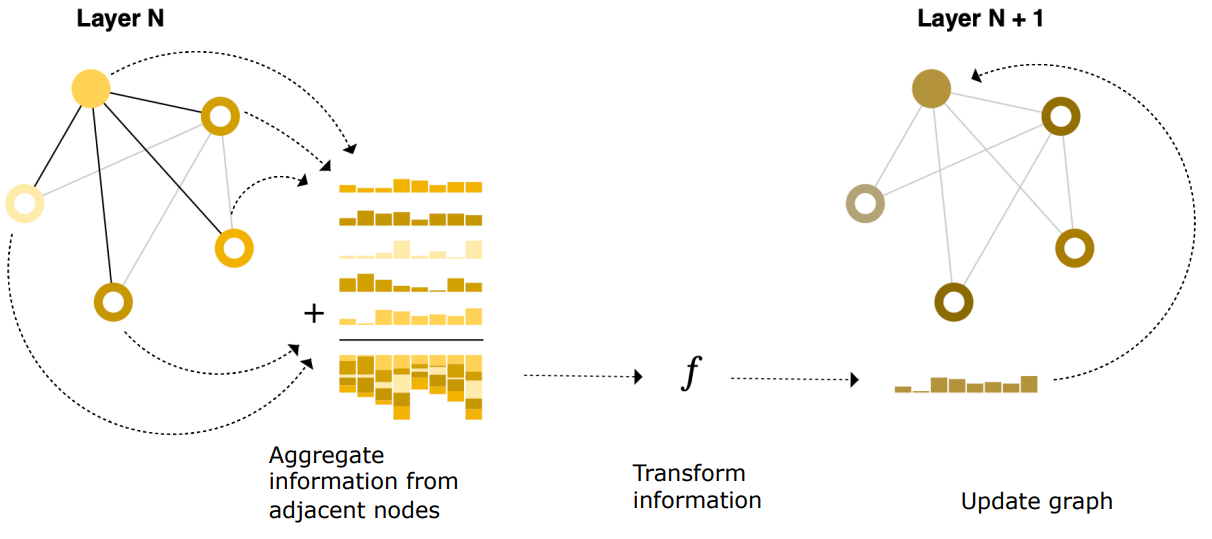
\includegraphics[width = \columnwidth]{figures/GraphNeuralNetworks1/MessagePassing.png}
\end{figure}
\begin{itemize}
    \item Simple GNN operation similar to CNNs, information is updatde with information obtained from neighbors
    \item The number of neighboring nodes can be variable in a graph
    \item The aggregation function must be specified accordingly, for example, sum or averaging are common
    \item By stacking message passing, a node can incorporate information from nodes further away
\end{itemize}
\subsubsection{Simple Message Passing}
\begin{figure}[!h]
    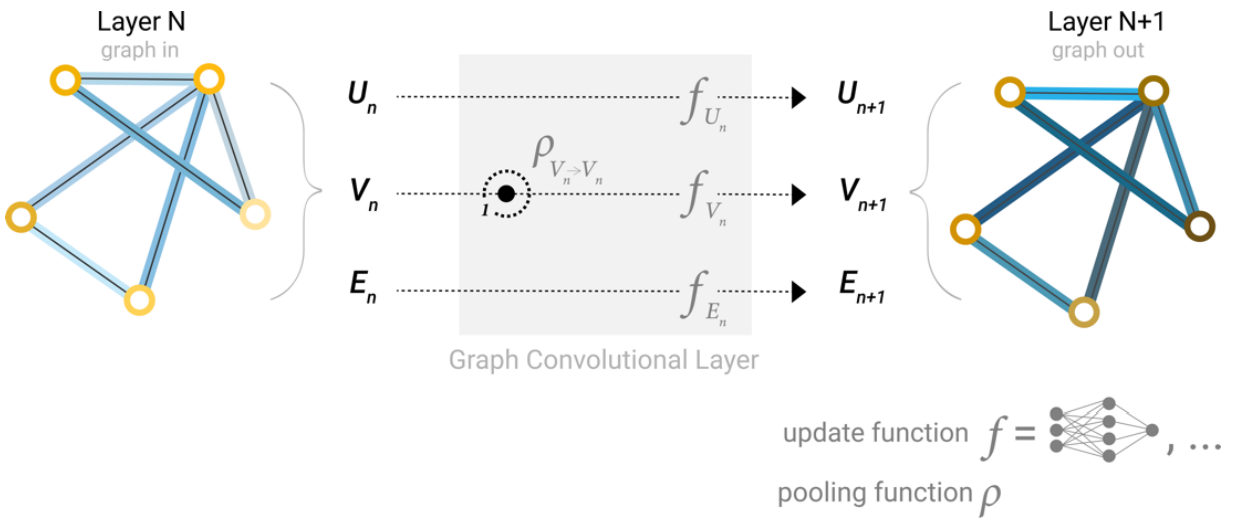
\includegraphics[width = \columnwidth]{figures/GraphNeuralNetworks1/SimpleMessagePassing.png}
\end{figure}